%\documentclass{book}\usepackage{sjtfonts}\usepackage{includegraphics}\usepackage{alltt}\usepackage{latexsym}
%\usepackage{array}
%\begin{document}\input{defs0}%		miradefs.tex 		    June 1994

% opening and closing a quoted Miranda section

\newcommand{\mira}{\noindent\hrulefill\nopagebreak\so}
\newcommand{\arim}{\nopagebreak\st\hrulefill\\}

% backslash in the Miranda environment
% Only feasible approach is to use \verb+\+
% in line!

%\newcommand{\bs}{$\mi\backslash\!\!$}
%\newcommand{\lbs}{\mbox{\verb+\+}}

% ignoring part of the input

\newcommand{\ignore}[1]{}

% a blank line in a Miranda section

\newcommand{\bl}{\mbox{\ }}

% Signalling a diffculty.

\definecolor{light-gray}{gray}{0.95}

\newcommand{\beware}[2]
 {\medskip\noindent\colorbox{light-gray}{\parbox{\textwidth}
 {\mbox{\large\textbf{#1}} \medskip\noindent\\ #2}\medskip\noindent}}

% Subscripting in Miranda text
\newcommand{\subscr}[2]{\mbox{${\mbox{\texttt{#1}}}_{\mbox{\texttt{#2}}}$}}

%\newcommand{\subscr}[2]{\mbox{${\mbox{\mi #1}}_{\mbox{\smtt #2}}$}}
\newcommand{\aone}{\subscr{a}{1}}
\newcommand{\atwo}{\subscr{a}{2}}
\newcommand{\ak}{\subscr{a}{k}}

\newcommand{\aoneone}{\subscr{a}{1,1}}

\newcommand{\eone}{\subscr{e}{1}}
\newcommand{\etwo}{\subscr{e}{2}}
\newcommand{\ei}{\subscr{e}{i}}
\newcommand{\er}{\subscr{e}{r}}

\newcommand{\fone}{\subscr{f}{1}}
\newcommand{\fl}{\subscr{f}{l}}

\newcommand{\gone}{\subscr{g}{1}}
\newcommand{\gtwo}{\subscr{g}{2}}
\newcommand{\gi}{\subscr{g}{i}}
\newcommand{\gr}{\subscr{g}{r}}

\newcommand{\hone}{\subscr{h}{1}}
\newcommand{\hl}{\subscr{h}{l}}

\newcommand{\pone}{\subscr{p}{1}}
\newcommand{\ptwo}{\subscr{p}{2}}
\newcommand{\pk}{\subscr{p}{k}}

\newcommand{\qone}{\subscr{q}{1}}
\newcommand{\qtwo}{\subscr{q}{2}}
\newcommand{\qk}{\subscr{q}{k}}

\newcommand{\rone}{\subscr{r}{1}}
\newcommand{\rtwo}{\subscr{r}{2}}

\newcommand{\tone}{\subscr{t}{1}}
\newcommand{\ttwo}{\subscr{t}{2}}
\newcommand{\tn}{\subscr{t}{n}}

\newcommand{\vone}{\subscr{v}{1}}
\newcommand{\vtwo}{\subscr{v}{2}}
\newcommand{\vn}{\subscr{v}{n}}

% for regular expressions

\newcommand{\stone}{\subscr{st}{1}}
\newcommand{\sttwo}{\subscr{st}{2}}
\newcommand{\stn}{\subscr{st}{n}}
\newcommand{\rthree}{\subscr{r}{3}}

\newcommand{\eps}{$\varepsilon$}
\newcommand{\trans}[1]{\stackrel{\mbox{\tt #1}}{\longrightarrow}}



% superscript in Miranda text

\newcommand{\superscr}[2]{\mbox{${\mbox{\mi #1}}^{\mbox{\smtt #2}}$}}

% Not equals in Miranda text

\newcommand{\noteq}{\makebox[0pt][l]{=}/}
\newcommand{\overslash}{\makebox[0pt][l]{/}}

% Definitions in complexity chapter

\newfont{\oldSym}{cmsy10}
\newcommand{\Th}{\boldmath$\oldSym\Theta$}
\newcommand{\pow}[1]{\^{}#1}
\newcommand{\leqq}{$\leq$}
\newcommand{\geqq}{$\geq$}
\newcommand{\lll}{$\ll$}
\newcommand{\eqq}{$\equiv$}
\newcommand{\ltwo}{\subscr{log}{2}}

% Indexing

\newcommand{\minx}[1]{\index{#1@{\ttfamily{}#1}}}
\setcounter{chapter}{19}\setcounter{page}{415}

%\minitocoptionfalse
\chapter{Conclusion}
\chapstart
\label{conclusion}

This book has covered the basics of functional programming
in the lazy language Haskell. It has shown how to craft programs, both by giving 
extensive examples as each new aspect of the language was introduced, and also by giving 
a series of larger case studies that run through the book. 

\section*{The power of functional programming}\index{functional programming!advantages of}
A functional programmer models the real world at a high level of
abstraction, concentrating on what relationships there are between
values, embodied in function definitions. This contrasts with a 
lower-level view  in which the details of how items are related predominate.
For instance, in Haskell lists are simply values, whereas in C or C++ they
become data structures built from pointers, and even in Java or C\# it is
difficult to present a suitably abstract model of lists.
This higher-level approach has a number of consequences, which have come out in the course
of the book.
\begin{itemize}

\item Higher-order functions and polymorphism combine to support the
construction of general-purpose libraries of functions, such as the list
functions in the Haskell standard prelude and library. The \texttt{map}
function, for instance,
\begin{alltt}
map :: (a -> b) -> [a] -> [b]
\end{alltt}
embodies the `pattern' of applying the same transformation to every
element in a list, which will be \textbf{reused} in a host of applications of
lists.
\itempar
Also supporting reuse through \textbf{overloading} are type classes, used for
instance in giving the function
\begin{alltt}
elem :: Eq a => a -> [a] -> Bool
\end{alltt}
which tests for membership of a list using the overloaded equality
function.

\item The definitions of functions are equations which express
properties of the functions defined. We can also express other properties of functions in a similar way. For example, we can relate 
\texttt{map} and
function composition, `\texttt{.}', by saying that  for all functions \texttt{f} and \texttt{g},
\begin{alltt}
map (f . g) ==  map f . map g
\end{alltt}
We can get \emph{strong evidence} that this property holds by testing it for randomly generated values of \texttt{f} and \texttt{g} using QuickCheck. 

\noindent
If we want to do some more work, we can \emph{prove} this property from the definitions of \texttt{map} and composition. 
Proof provides a user with assurance about how a program behaves on all arguments,
in contrast to testing which can only give direct information about its
behaviour on a (hopefully) representative selection of inputs.

\item Data structures can be introduced in a directly recursive manner,
giving trees, queues and so forth without having to look at their
representations. Algorithms are written at the same level as they would
be described informally, in contrast with more traditional approaches
which make the representation very clear.

\item Pulling all this together, we can use these and other facilities of Haskell to build implementations of domain-specific languages (DSLs) embedded in Haskell. These DSLs allow users to express problems and models in a language appropriate to the domain, but at the same time to use all the power of Haskell when necessary.

\end{itemize} 
A text like this can only provide an introduction to a subject as rich
and developed as functional programming; the rest of this concluding
chapter discusses other aspects of the subject, as well as giving pointers to 
other sources on the Web and in books and articles.

\section*{Further Haskell}
\index{Haskell!further features}

The purpose of this text is to introduce functional programming ideas using the
Haskell language. It covers the important aspects of the language, but does not
aim to be complete. Among the topics omitted are data types with labelled fields, which resemble
records or structures in other languages; strictness annotations, 
which are used to make data type constructors strict in some or all of their arguments; 
details of the \texttt{Read} class and the numeric types and classes. 

Further information about all these
can be found in the Haskell language report  \cite{haskell2010}, and the
`Gentle Introduction' of \cite{gentle98} also contains useful
information about some of them, as well as providing an
overview of the language for an experienced functional programmer. Both
of these, as well as many other Haskell resources, can be found at the
Haskell home page, \texttt{http://www.haskell.org/}.

Where can you go to find out what to do next in Haskell? Again the \texttt{haskell.org} site has many links, but three specific things you might like to look at are 
\begin{itemize}\index{Haskell!what to read next}
\item
\emph{Real World Haskell} \cite{realWorldHaskell} which is available in print and also online.  It starts from the beginning, but goes at a faster pace than we did here, and so covers a number of practical aspects of Haskell which we weren't able to do, such as the foreign function interface. So, it's the perfect follow-on read.
\item
\emph{Learn You a Haskell for Great Good!} \cite{learnYou} is a website and soon to be a printed book which introduces Haskell for those who are familiar with imperative programming. It's written in a very approachable style, and complements what we have covered here, as well as going into some topics -- like monads and zippers -- in much more detail.
\item
\emph{Pearls of Functional Algorithm Design} \cite{BirdPearls} this delightful book looks at a series of 30 problems, and solves them using the \emph{design by calculation} approach, which is ideally suited to writing functional programs in Haskell.
\end{itemize}
The text has discussed many of the most important functions in the
standard prelude but on the whole has avoided discussing the contents
of the libraries in detail. As we explained in Chapter \ref{progLists}, they are documented in Haddock, and this documentation is available online for type- and name-based search in Hoogle. Moreover, the packages in Hackage are themselves documented and have information available in Hayoo.

\subsection*{The future of Haskell}
\index{Haskell!prospects}

Haskell was first defined in 1987, and has been modified and extended a number of times
since then. This text is written in Haskell 2010,\index{Haskell 2010} which is meant to
provide a stable base system consisting of tried and tested features.

The progress of research in functional programming makes it clear that a
language like Haskell will not stand still, and Haskell is now undergoing regular language standard updates. These are set to incorporate features which have become \emph{de facto} parts of the language through their implementation in GHC, as well as more advanced features, particularly in the type system.
The Haskell home page
can be relied upon to contain up-to-date information on the status of Haskell.

\begin{figure}[t]
\begin{center}
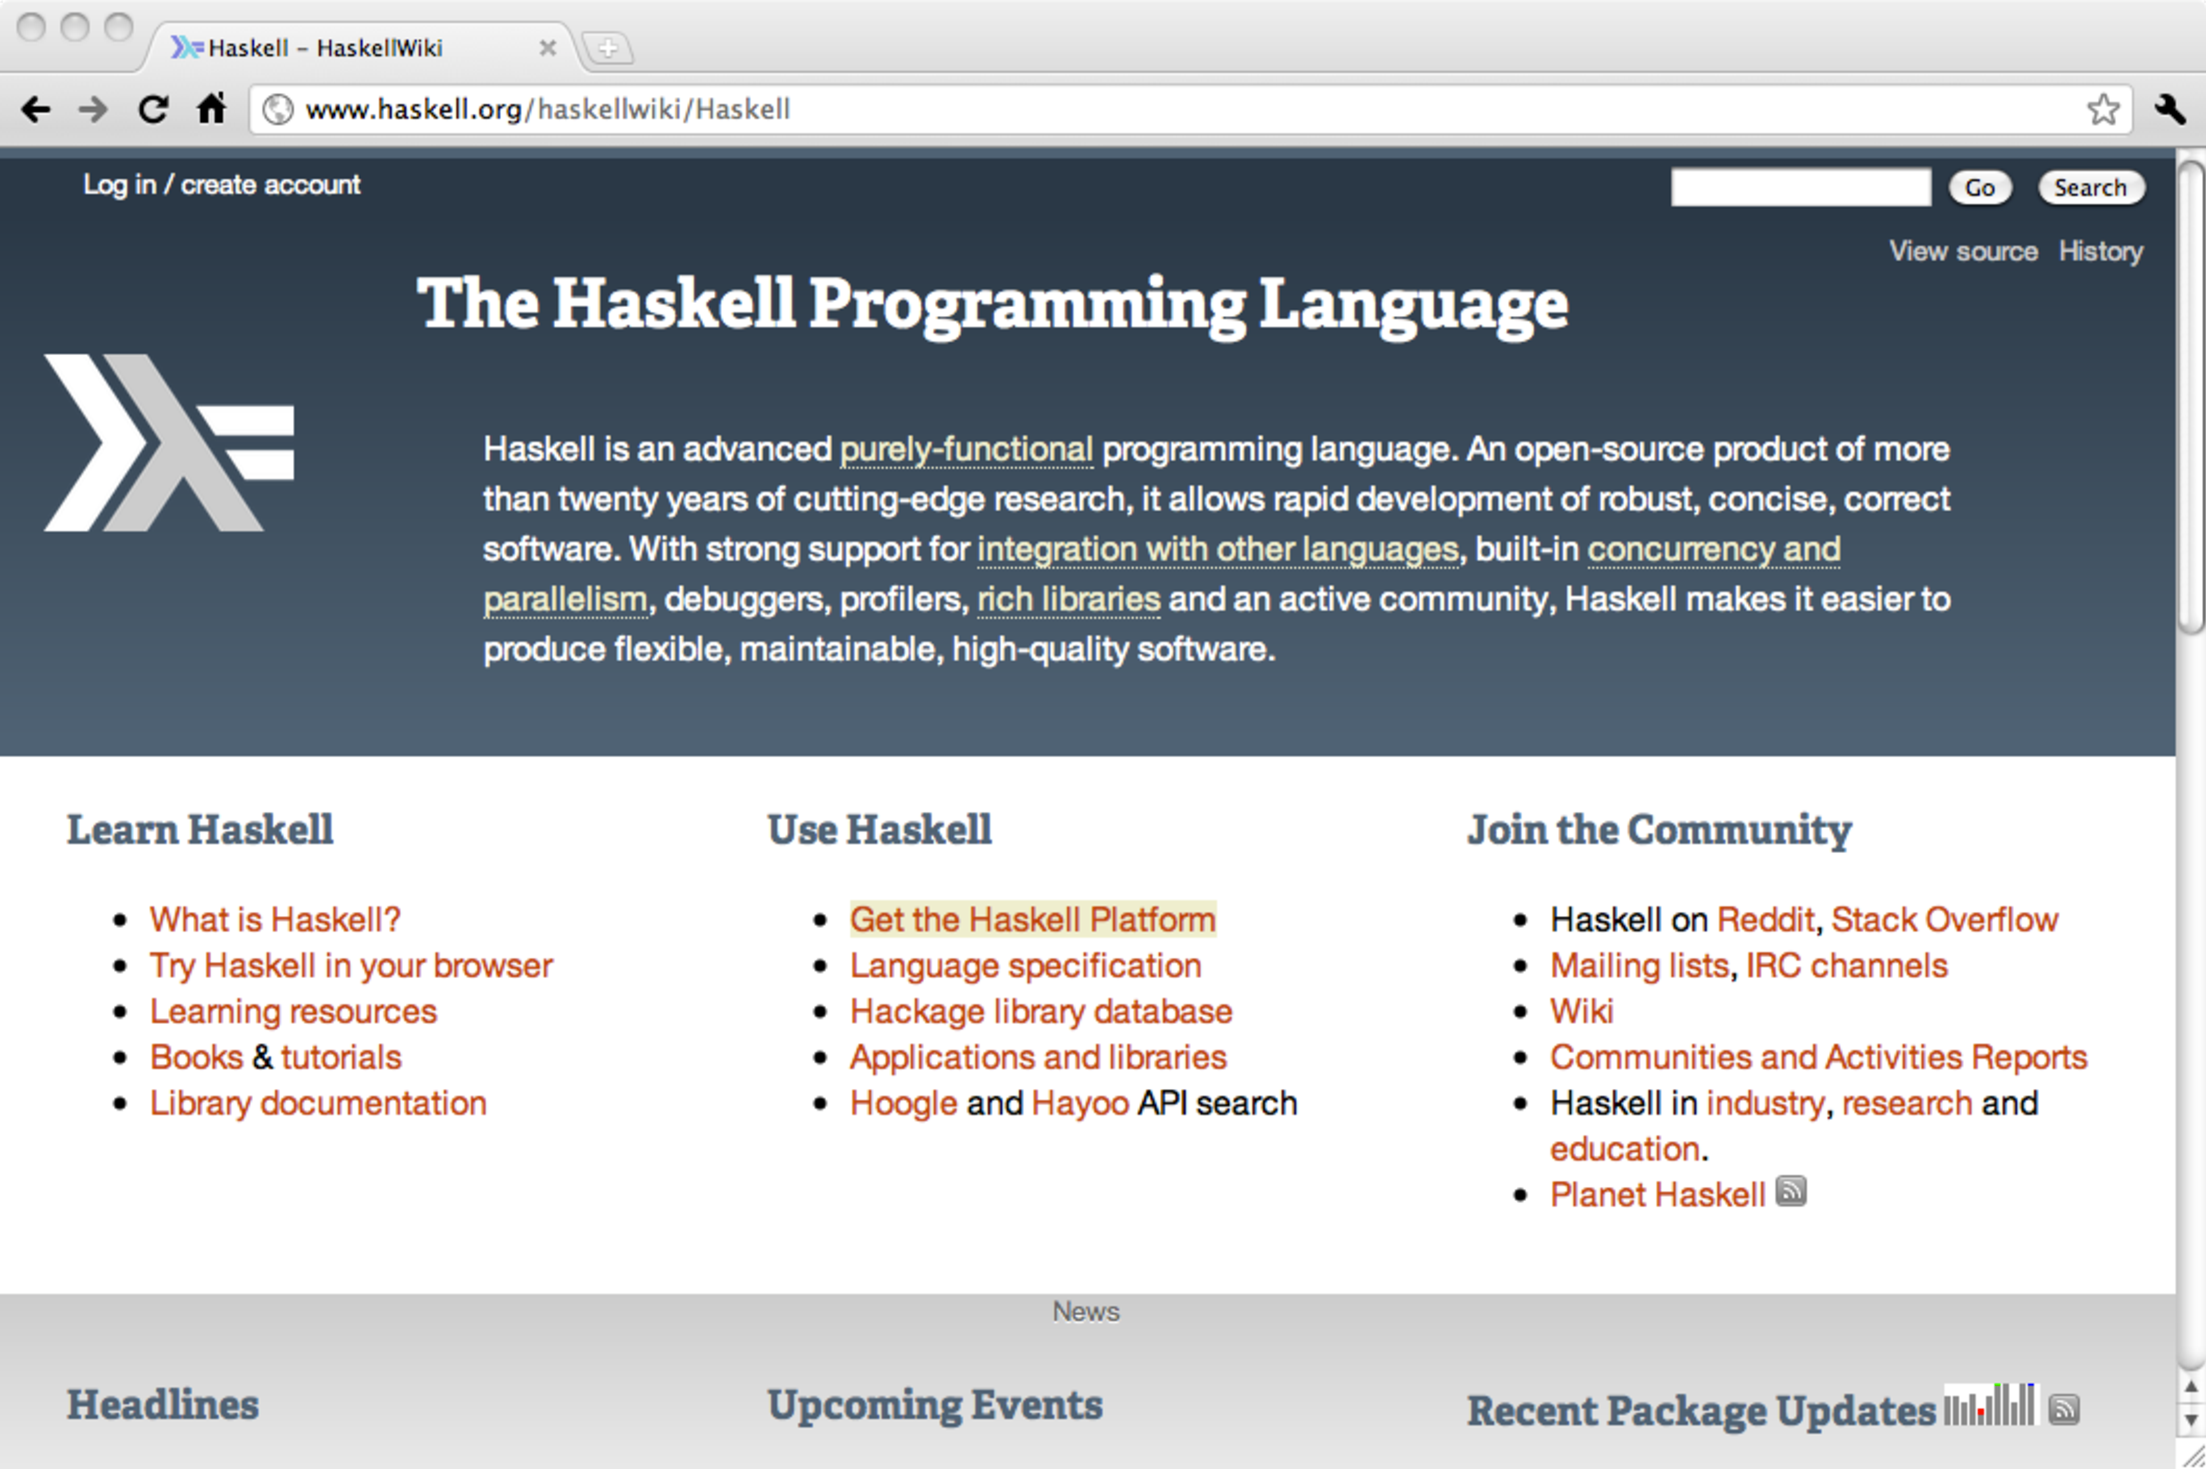
\includegraphics[width=5in]{Pictures/HaskellDotOrg.pdf}
\end{center}
\caption{The Haskell home page, \texttt{www.haskell.org}}
\label{HaskellDotOrg}
\end{figure}

\section*{Haskell on the web}
\index{Web site!sites with further information}

There are now many resources on Haskell and functional programming to be
found on the wbe. This text itself has a home page at
\begin{alltt}
www.haskellcraft.com
\end{alltt}
which lists all the links given here.
The Haskell home page, Figure \ref{HaskellDotOrg}, is at
\begin{alltt}
http://www.haskell.org/
\end{alltt}
and that should be your first stop for everything to do with Haskell. As you can see from the figure, the home page has links to learning resources, to documentation about libraries and packages, and to the wider Haskell community. 

The Haskell community includes online forums (IRC, mailing lists), news (Reddit), blogging (Planet Haskell) and help (Stack Overflow). The Haskell Communities and Activities reports provide a biannual snapshot of what's going on with Haskell: the most recent edition is 77 (two-column, A4) pages long, and contains a wealth of detail on who is doing what with Haskell. Subscribers to Planet Haskell or the mailing lists also receive Haskell Weekly News, which summarises Haskell-related software releases, blog entries and other news.

The Haskell language was named in honour of Haskell Brooks Curry. A
short biography and photograph of Curry can be found at\index{Curry,
Haskell B.!biography}
\begin{alltt}
http://www-history.mcs.st-and.ac.uk/Biographies/Curry.html
\end{alltt}

\section*{Other functional programming languages}\index{functional programming!other languages}

Haskell is a lazy, strongly typed functional programming language; 
another is Miranda \cite{mira,miraCraft}.\index{Miranda} In
this text laziness is only examined explicitly in Chapter \ref{lazy},
and up to that point it looks at aspects of functional programming which
are broadly shared with Standard ML\index{Standard ML} \shortcite{defsml2e,mlCritique}, the
best known and most widely used strict and strongly typed functional language, for which
\citeN{workingml2e} provides an introduction. The latest member of the ML family of languages, is F\# \cite{Fsharp}, which is distributed by Microsoft as a part of Visual Studio 2010. Since is possible to model
lazy evaluation within a strict language, and Haskell provides
facilities to make evaluation strict, the Haskell and ML schools of programming are very close
indeed.

A different style of functional programming, `point-free programming', eschews variables as much
as possible: this was introduced in \citeN{backus}. \citeN{AoP} is a text that
emphasizes the benefits of this style in supporting program
transformation and also advocates a `relational' style of programming
which extends the functional.

LISP is the oldest established functional language, but it differs from
Haskell and SML in not being strongly typed. An excellent tutorial
introduction to programming in the Scheme\index{Scheme} dialect of LISP is given in 
\citeN{strAndInterp}. \emph{Land of Lisp} \cite{LandOfLisp} is a book, website and music video\footnote{\ldots simple but refined, guaranteed to blow your mind \ldots} introducing Lisp by developing a series of games.
 
Erlang is a concurrent, fault-tolerant, distributed language, based on a functional programming core. Erlang \cite{progErlang,erlangProg} was developed within Ericsson, and as well as its use in telecoms applications, has applications in the financial sector, and to high-availability distributed systems in general. 

Two surveys of applications of functional programming languages in
large-scale projects are \citeN{applicsFP} and \citeN{stateArtFP}, and
there is also up-to-date information about this at the Haskell home page.

Over the last two decades, powerful techniques of implementation of especially
lazy functional languages have been developed. The twin texts
\cite{pj,pj-lester} describe the foundations of these in lucid detail.

\section*{Where is functional programming going?}\index{functional programming!future direction of}

The material in this text is an introduction to modern functional
programming in a typed, lazy, language. As the field develops, new
techniques and approaches are continually being developed; a good place
to start in learning about these is by looking at the proceedings of a series of summer
schools in Advanced Functional Programming
\cite{advancedFP,advancedFP2,advancedFP3,advancedFP4,advancedFP5,advancedFP6}. 

Research in functional programming is reported in the {\em Journal
of Functional Programming}
\begin{alltt}
http://journals.cambridge.org/jfp
\end{alltt} 
and at the annual
International Conference in Functional Programming, 
\begin{alltt}
http://www.icfpconference.org/
\end{alltt} 
Each year there is a one-day symposium devoted to research in Haskell, 
\begin{alltt}
www.haskell.org/haskell-symposium/
\end{alltt}
and the proceedings of this symposium (formerly workshop) will give you a view of the direction in which Haskell is going. 
The symposium is co-located with ICFP, as is the meeting of CUFP,
\texttt{cufp.org},
which represents Commercial Users of Functional Programming.

To see the ways in which functional
languages are being used in education, the proceedings of a meeting on
Functional Languages in Education appear in \citeN{fple95}, and these
have been followed up with a series of occasional workshops co-located with ICFP.

It is difficult to predict future directions in a field like computing. In the previous edition of this book (written 1998--9) I predicted three things:
\begin{itemize}
\item functional languages will come to be used as parts of larger systems;
\item type systems for languages like Haskell will become more powerful and esoteric, and
\item tool support, for instance giving feedback on the behaviour of lazy programs, will come to maturity.
\end{itemize}
Not a bad set of predictions. The first is certainly true, with Haskell inter-operating effectively with a range of other languages through its foreign function interface. GCH continues to be a laboratory for type system research, with recent advances in type-level programming taking it ever closer to dependently-typed languages such as Agda,\index{Agda}\index{type!dependent types}
\begin{alltt}
http://wiki.portal.chalmers.se/agda/
\end{alltt}
Tool support for Haskell has also come of age, with many tools integrated into GHC, and it becoming easier for others to integrate their work through the definition of an API for the internals of GHC. What I had not predicted was the growth in the Haskell developer community: fuelled particularly by Hackage and Cabal, making it easy to share and to work collaboratively, there are now close to three thousand projects on Hackage, giving the developer community a critical mass which was entirely lacking a decade ago.\footnote{It was also a surprise that Microsoft started to deploy a functional language as a part of their main language suite in Visual Studio: a friend mailed me and said that his first thought it was an `April fool' message, even though it came in June!} 

What of the next few years? The big challenge for systems developers is the rise of multicore chips: chips with thousands of processors are on the roadmap, and so the question arises of how best to program them, or indeed how to program them at all! Functional languages, because of their lack of side-effects, and clean models for concurrency, make them ideal candidates for the next generation of general purpose languages for multicore. The next few years will be fascinating, and of course, unpredictable, but it will be a surprise if functional languages are not playing a much more important role in robust software development in ten years time, with Haskell central to this achievement.


%\end{document}
